\clearpage
\begin{flushright}
	\textit{Лекция №23}
	\textit{2015.12.15}
\end{flushright}

\begin{figure}[H]
    \centering
    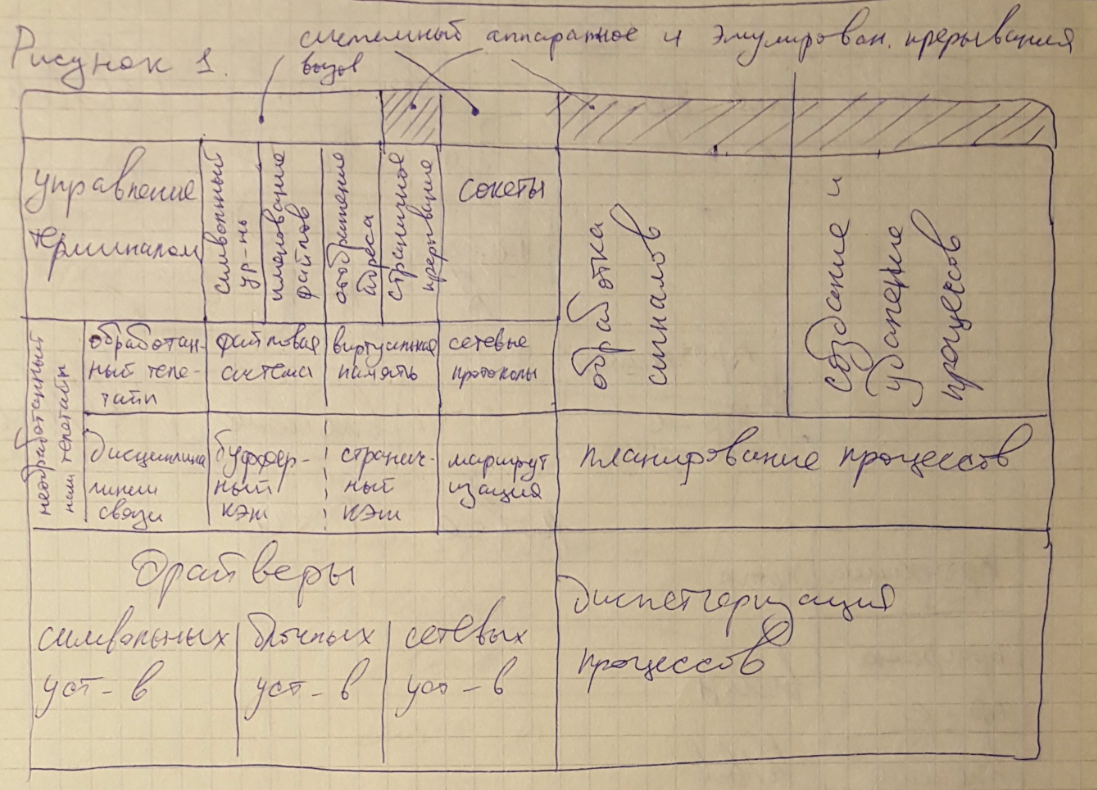
\includegraphics[width=\textwidth]{pic/1.png}
    \caption{Структура ядра QNX 4.4 BCD}
\end{figure}

Иерархическая организация с монолитным ядром. Все уровни показывают, что остается в микроядре, и что остается режиме пользователя. Она базируется на Unix.
Планирование – постановка процессов в очередь в соответствии с их приоритетами.
Диспетчеризация – непосредственное выделение кванта процессорного времени.
Драйверы – для управления внешними устройствами.
Сокеты – средство взаимодействия процессов в Linux BCD.

\chapter{Прерывания}

Существуют 2 подхода к реализации обработки прерываний в системе:
\begin{enumerate}
    \item запрет прерываний на время выполнения обработчика прерывания. Запрет прерываний на длительное время в системе – невозможен. Поэтому обработчики прерываний делятся на быстрые и медленные, а медленные делятся на две части: верхнюю и нижнюю половину. Обработчик таймера может инициализировать последующее выполнение планировщика выполнения. Верхняя половина считывает в буфер информацию из контроллера и заканчивается инициализация последующего выполнения нижней половины обработчика. В Юникс поддерживается несколько типов вторых половин. В winows тоже самое, но через DPC.
    \item вложенные прерывания.
\end{enumerate} 

\paragraph{Вложенные прерывания}

\begin{figure}[H]
    \centering
    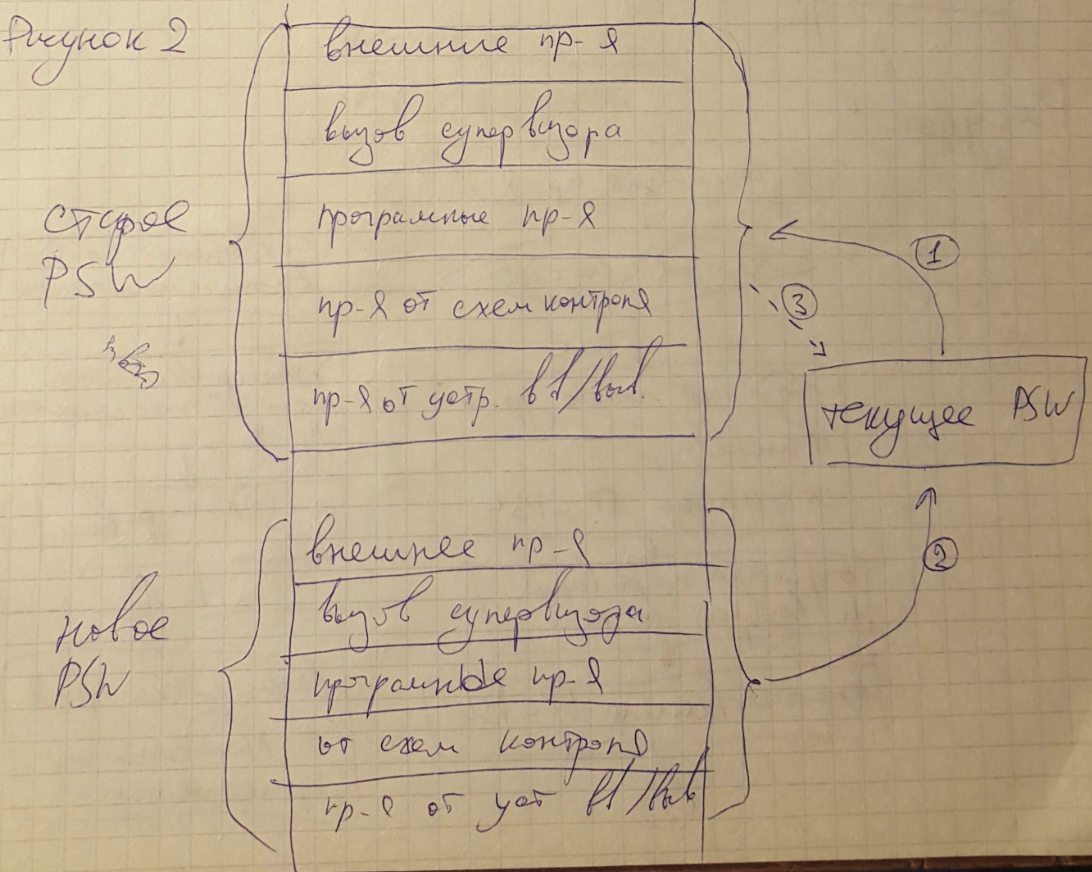
\includegraphics[width=\textwidth]{pic/2.png}
    \caption{pic}
\end{figure}

PSW - аппаратный контекст. 

Механизм прерывания реализуется аппаратно (шаги):
\begin{enumerate}
    \item текущее PSW записывается в место старого PSW
    \item новое PSW загружается в качестве текущего
    \item по завершению обработки прерывания старое PSW загружается в место текущего, что дает возможность продолжить выполнение прерванной программы.
\end{enumerate} 

Пример: пусть одновременно возникло три сигнала прерывания:
\begin{enumerate}
    \item программное прерывание (5 приоритет)
    \item внешнее (3)
    \item устройств ввода/вывода (2)
\end{enumerate} 

\begin{figure}[H]
    \centering
    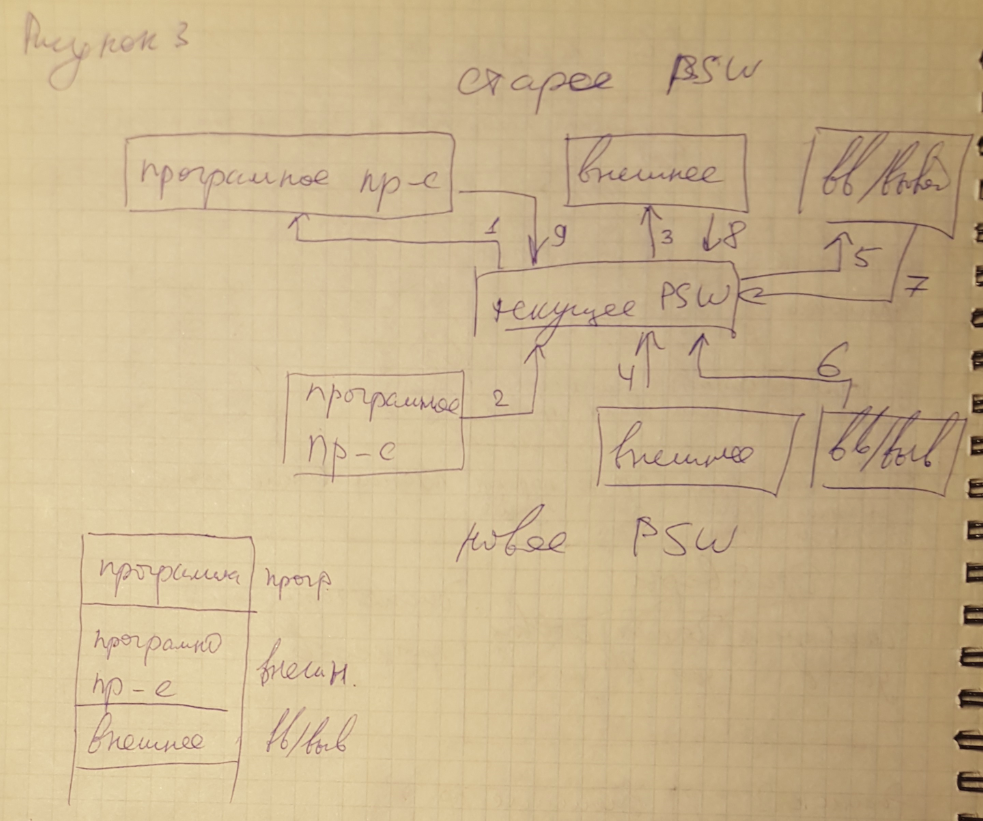
\includegraphics[width=\textwidth]{pic/3.png}
    \caption{pic}
\end{figure}

Процесс обработки прерывания. Аппаратные прерывания. Основная функция аппаратных прерываний – информировать процессор о завершения операций ввода/вывода, что позволяет процессору отключиться на какое то время от управления устройством (распараллеливание функций). Это асинхронные события. Система не знает, в каком месте выполнения потока инструкций произойдет прерывание. В результате прерывания в системах х86 через таблицу дескрипторов прерываний осуществляется вызов соответствующего обработчика прерываний, называемый ISR (interrupt service routine). Выполняется в режиме ядра в системном контексте, так как прерванный процесс не имеет отношения к возникшему прерыванию, обработчик этого прерывания не должен обращаться к контексту процесса. По этой причине он не обладает правом блокировки. Прерывание все равно оказывает некоторое влияние на выполнение текущего процесса, а именно, время потраченное на обработку прерывания является частью выделенного процессу кванта. Обработчик прерывания системного таймера использует тики текущего процесса и поэтому нуждается к доступу к его структуре proc. Контекст процесса не полностью защищен от доступа к адресному пространству процесса. 

Прерывания могут возникнуть в результате возникновения множества независимых событий в системе. Поэтому реальна ситуация, когда во время одного прерывания, возникает другое. При этом прерывание аппаратного таймера должно обслуживаться сразу. Вводится поддержка различных уровней приоритета Interrupt priority level. Уровни IPL сравниваются и устанавливаются на аппаратном уровне. Ядро может повысить приоритет некоторых критических инструкций. На некоторых аппаратных платформах поддерживается глобальный стек прерываний, используемый всеми обработчиками. На платформах, не имеющих такого стека, задействуют стек ядра текущего процесса. Должен быть обеспечен механизм изоляции стека ядра от обработчика. Ядро помещает в стек уровень контекста перед вызовом обработчика. 

\paragraph{Алгоритм обработки прерывания}

\begin{figure}[H]
    \centering
    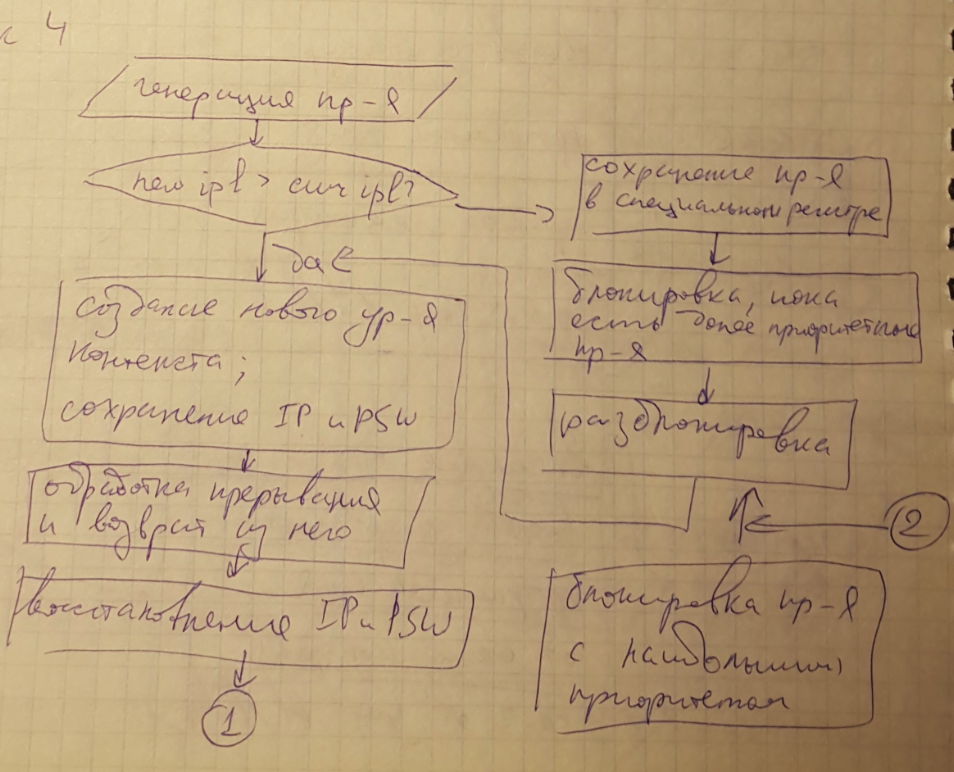
\includegraphics[width=\textwidth]{pic/4.png}
    \caption{Алгоритм обработки прерывания}
\end{figure}

\begin{figure}[H]
    \centering
    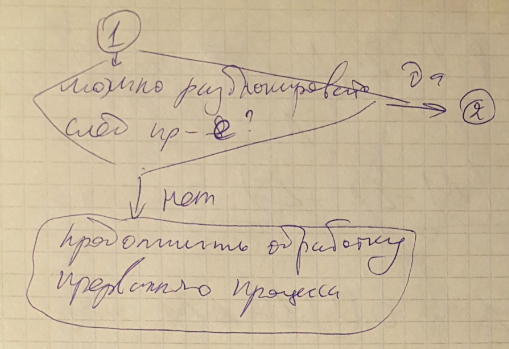
\includegraphics[width=\textwidth]{pic/5.png}
    \caption{Алгоритм обработки прерывания}
\end{figure}

Обработчики прерываний входят в состав драйверов соответствующих устройств. Они регистрируются в этих драйверах. 

\paragraph{Реализация обработки прерываний в Windows.}

Завершая передачу данных, контроллер устройства генерирует прерывание. Это прерывание в х86 приходит на выделенную ножку контроллера прерываний. После того, как прерывание получено, начинает действовать ядро, а именно диспетчер ввода/вывода и драйвер устройств. В результате процессор передает управление (в windows обработчик ловушки ядра или ISR) в соответствии с таблицей диспетчеризации прерываний. 

ISR в windows выполняется в два этапа: 

1 этап. На уровне device irql (на этом этапе сохраняется название устройства и запрещаются дальнейшие прерывания от него)\\
DPC – deferred procedure call (отложенный вызов процедуры).

\begin{figure}[H]
    \centering
    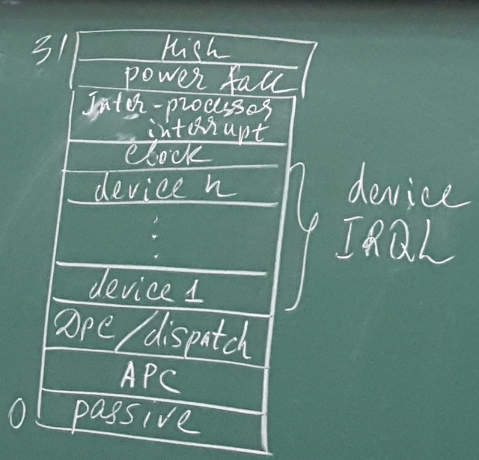
\includegraphics[width=\textwidth]{pic/6.png}
    \caption{pic}
    \label{pic:pic_lec23_1}
\end{figure}

2 этап. ISR помещает DPC в очередь на выполнение, после чего завершает прерывание и завершается.

\begin{figure}[H]
    \centering
    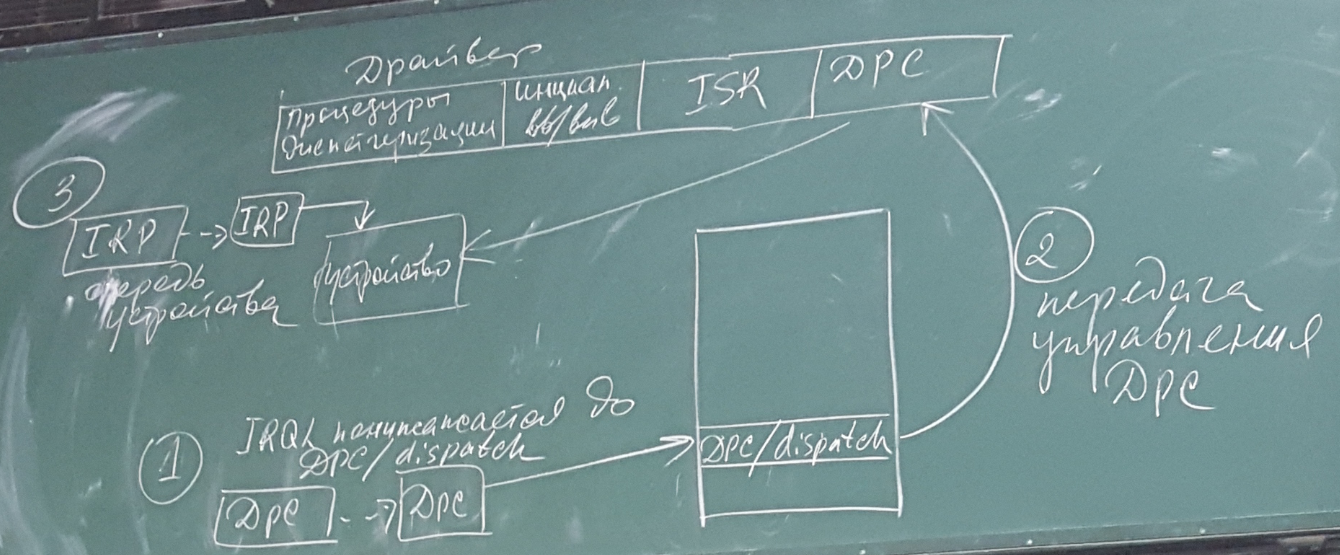
\includegraphics[width=\textwidth]{pic/7.png}
    \caption{pic}
\end{figure}

\begin{figure}[H]
    \centering
    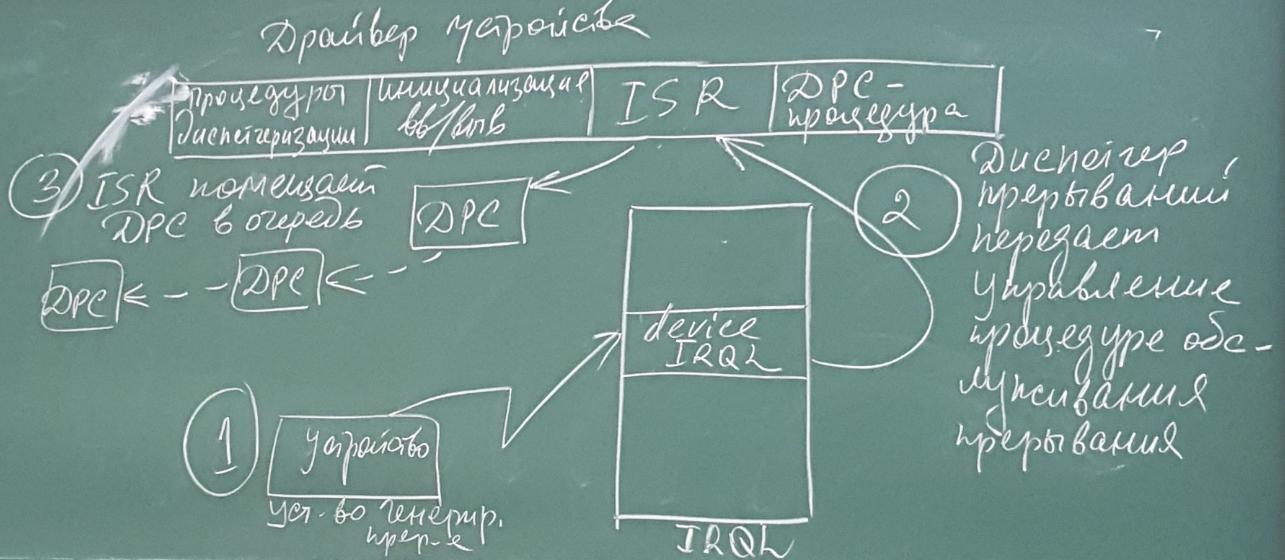
\includegraphics[width=\textwidth]{pic/8.png}
    \caption{Первая часть обработки}
\end{figure}

На первой фазе  устройство генерирует прерывание, определяется уровень данного прерывания irql, вызывается обработчик соответствующего прерывания ISR, который входит в состав драйвера. ISR должна выполнять минимум действий, связано это с тем, что часть действий – критические, и должны выполняться, как неделимые.  Основное действие – сохранение информации о состоянии прерывания. Второе действие – инициализация отложенного действия.
ДПС процедура начинает обработки следующего запроса из очереди устройства IRP (пакет), после чего заканчивает обработку прерывания. В системе столько очередей DPC, сколько процессоров. DPC – объект. По умолчанию ядро помечает DPC объекты в конец DPC очереди того процессора, на котором выполнялось ISR. Однако драйвер устройства может указать приоритет DPC {низкий, средний, высокий}, а также может направить DPC в очередь конкретного процессора.  Низкий - когда очередь DPC превышает пороговое значение. DPC применяется, когда истекает квант. При каждом тике системного таймера генерируется прерывание IRQL clock (приоритет его выше всех девайсов, это видно на \ref{pic:pic_lec23_1}. Обработчик прерывания таймера обновляет системное время и уменьшает квант. Когда счетчик кванта обнуляется, ядру может понадобиться перераспределить процессорное время. По \ref{pic:pic_lec23_1} задача перераспределения имеет ???. Обработчик прерывания таймера ставит DPC  в очередь для того, чтобы инициализировать диспетчеризацию потоков, после чего завершает свою работу и IRQL процессора понижается. По истечению кванта пересчитывать приоритеты – поздно. Оно осуществляется по главному тику. Таймер инициализирует постановкой соответствующего объекта DPC в очередь процессору. И когда обработчик таймера завершается, когда код обработчика прерывания завершился, IRQL процессора понижается. Сначала находилось на уровне clock. Power выше, чтобы система сохранила работоспособность,  всё завершается, выполняет сохранение состояний, чтобы потом могли сохранить работу. Если DPC имеет приоритет ниже приоритета всех аппаратных прерываний, то сначала обрабатываются все возникшие аппаратные прерывания, а затем генерируется прерывание DPC. На уровне passive могут выполняться некоторые потоки ядра и процессы пользователя.